
\documentclass[11pt]{article}
\PassOptionsToPackage{svgnames}{xcolor}
\usepackage{graphicx} % Required for inserting images
\usepackage[utf8]{inputenc}
\usepackage[margin=1in]{geometry}
\usepackage{enumerate, fancyhdr, color, verbatim, setspace, multirow, multicol,subcaption, booktabs, caption, amsfonts}
\usepackage{rotating}
\usepackage{amsmath}
\usepackage{amsthm}
\usepackage{listings}
\numberwithin{equation}{section}
\newtheorem{definition}{Definition}[subsection]
\newtheorem{theorem}{Theorem}[subsection]
\newtheorem{corollary}{Corollary}[subsection]

\usepackage{colortbl}
\usepackage{tikz}
\usetikzlibrary{matrix, positioning, shadings, shadows}
\usepackage{pgfplots}
\pgfplotsset{compat=1.18}
\usepackage[shortlabels]{enumitem}
% \usepackage[symbol]{footmisc}
\usepackage{multirow}
\usepackage{multicol}
% Creates the header and footer. You can adjust the look and feel of these here.
\usepackage{hyperref}
\hypersetup{
    colorlinks,
    citecolor=black,
    filecolor=black,
    linkcolor=blue,
    urlcolor=blue
}
\newcommand{\bp}{\mathbb{P}}

\definecolor{lightgray}{RGB}{230, 230, 230}
\definecolor{lightgrey}{RGB}{200, 200, 200}

\usepackage{tcolorbox}
\newenvironment{myblock}[1]{%
    \tcolorbox[beamer,%
    noparskip,breakable,
    colback=lightgray,colframe=black,%
    colbacklower=lightgrey,%
    title=#1]}%
    {\endtcolorbox}

\tcbuselibrary{skins,breakable}


\renewcommand{\headrulewidth}{0.2pt} %Creates a horizontal line underneath the header
\setlength{\headheight}{15pt} %Sets enough space for the header
% \renewcommand{\theenumi}{\alph{enumi}}
\onehalfspacing

\usepackage{chngcntr}
\counterwithin{figure}{section}

\DeclareMathOperator*{\argmin}{arg\,min}
\DeclareMathOperator*{\argmax}{arg\,max}

\usepackage[backend=biber, style=authoryear, maxcitenames=2, maxbibnames=9]{biblatex}
\DeclareDelimFormat{nameyeardelim}{\addcomma\space}
\addbibresource{references.bib}

\setcounter{tocdepth}{2}

\title{MGTECON 603 - Problem Set 1\\ \small{(Instructor: Guido Imbens)}}
\author{Wooyong Park\\ {\small Collaborators: Cem Kozanoglu, Roberto Gonzalez Tellez, Hanniel Ho, Aileen Wu}}
\date{\today}

\begin{document}


\maketitle

\section{Part I}

\subsection*{Descriptive Statistics}

The summary statistics of the data are shown in tables \ref{tab:summary_stats}, \ref{tab:summary_stats(control_group)}, and \ref{tab:summary_stats(treated_group)} in the appendix.

The histogram of the outcome variable \verb|earnings1yr| (Figure \ref{fig:hist_earnings1yr}) displays a heavily zero-inflated distribution, and overall we have more treated units than control units.

\begin{figure}[h]
    \centering
    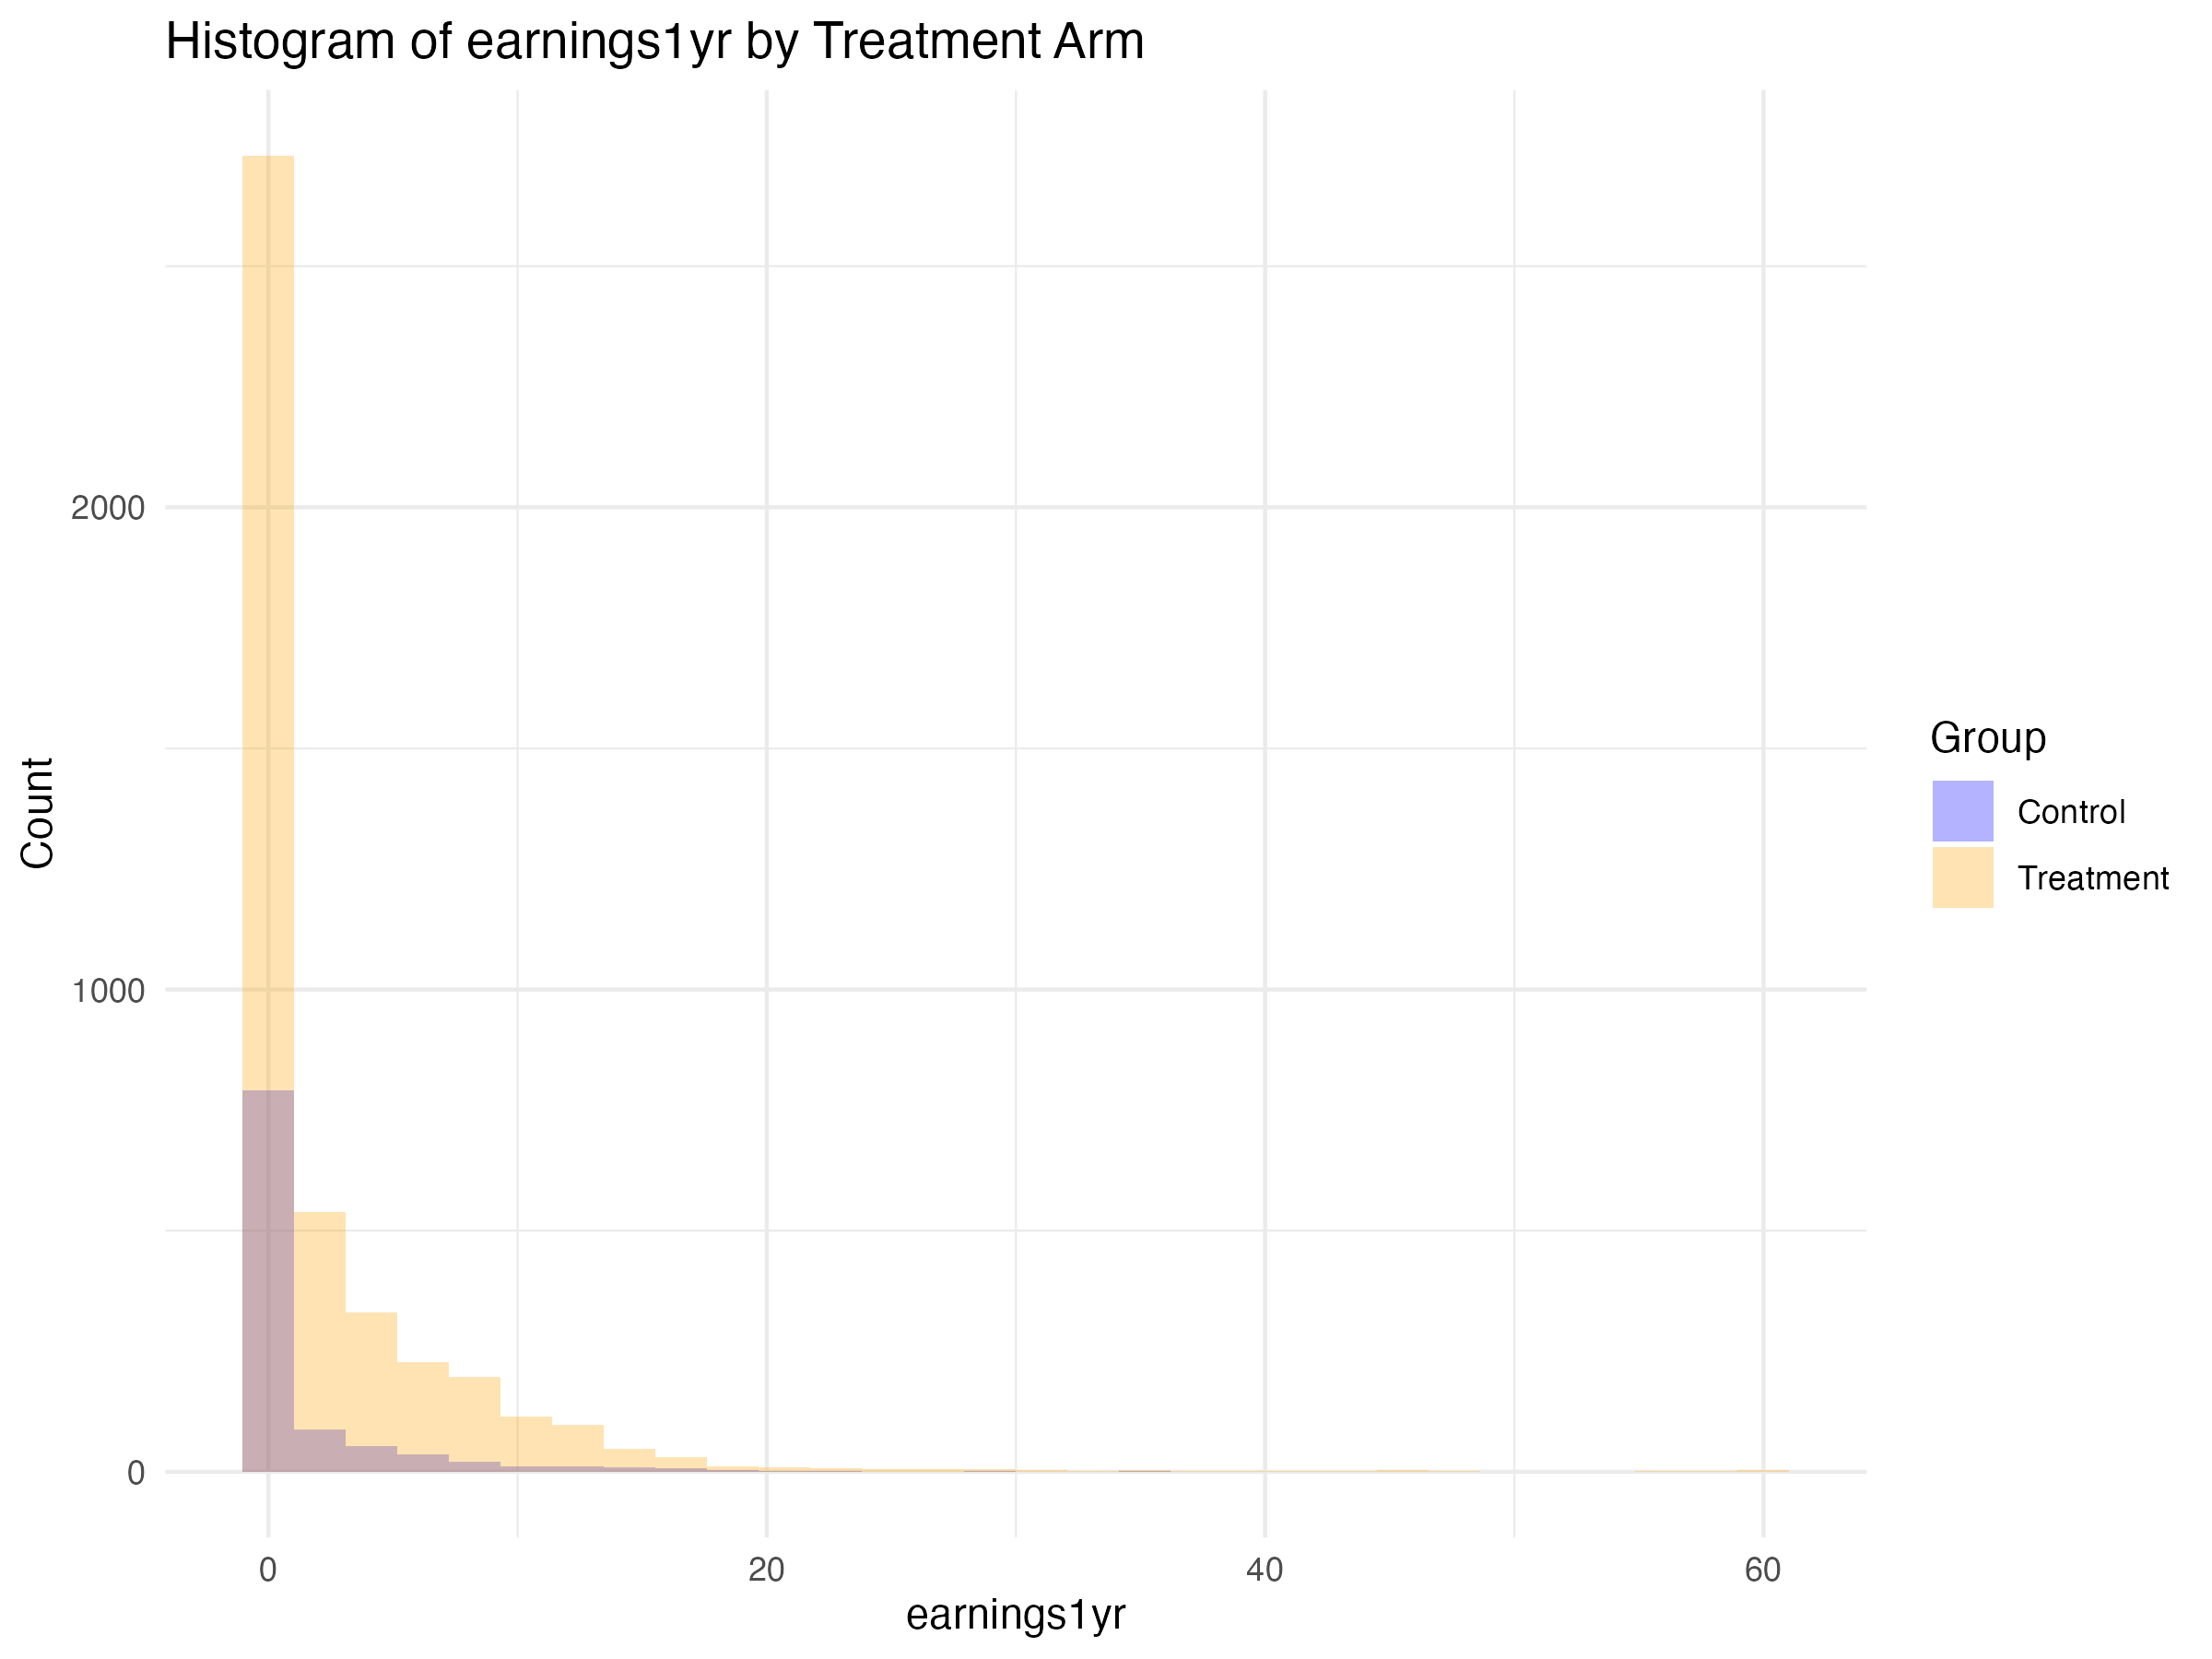
\includegraphics[width=0.8\textwidth]{output/histogram_earnings1yr_by_treatment_arm.png}
    \caption{\label{fig:hist_earnings1yr}Histogram of earnings1yr by treatment arm}
\end{figure}





\subsection*{(a) Difference-in-Means}

Assuming our data is not a random sample but the population itself, the number $M$ given in the problem must be the actual number treated in our dataset, which is 4,383. 
I create 99, 999, 9999, and 99999 random draws of treatment assignments with exactly 4,383 treated units to create the same number of test statistics that would be comparable to the actual test statistic.
 – In principle, I must have $\binom{n}{M}$ possible treatment assignments, but since this number is extremely large, I will only create at maximum 99,999 random draws, assuming that it is a large enough number so that the difference of the exact population p-value and the p-value that I have from the 99,999 random draws is negligible –
The reason I have multiple number of draws is to see if the p-value changes significantly. If I see histograms and p-values converging at some point, we might not need to increase the numbers of draws.



\begin{figure}[h]
    \centering
    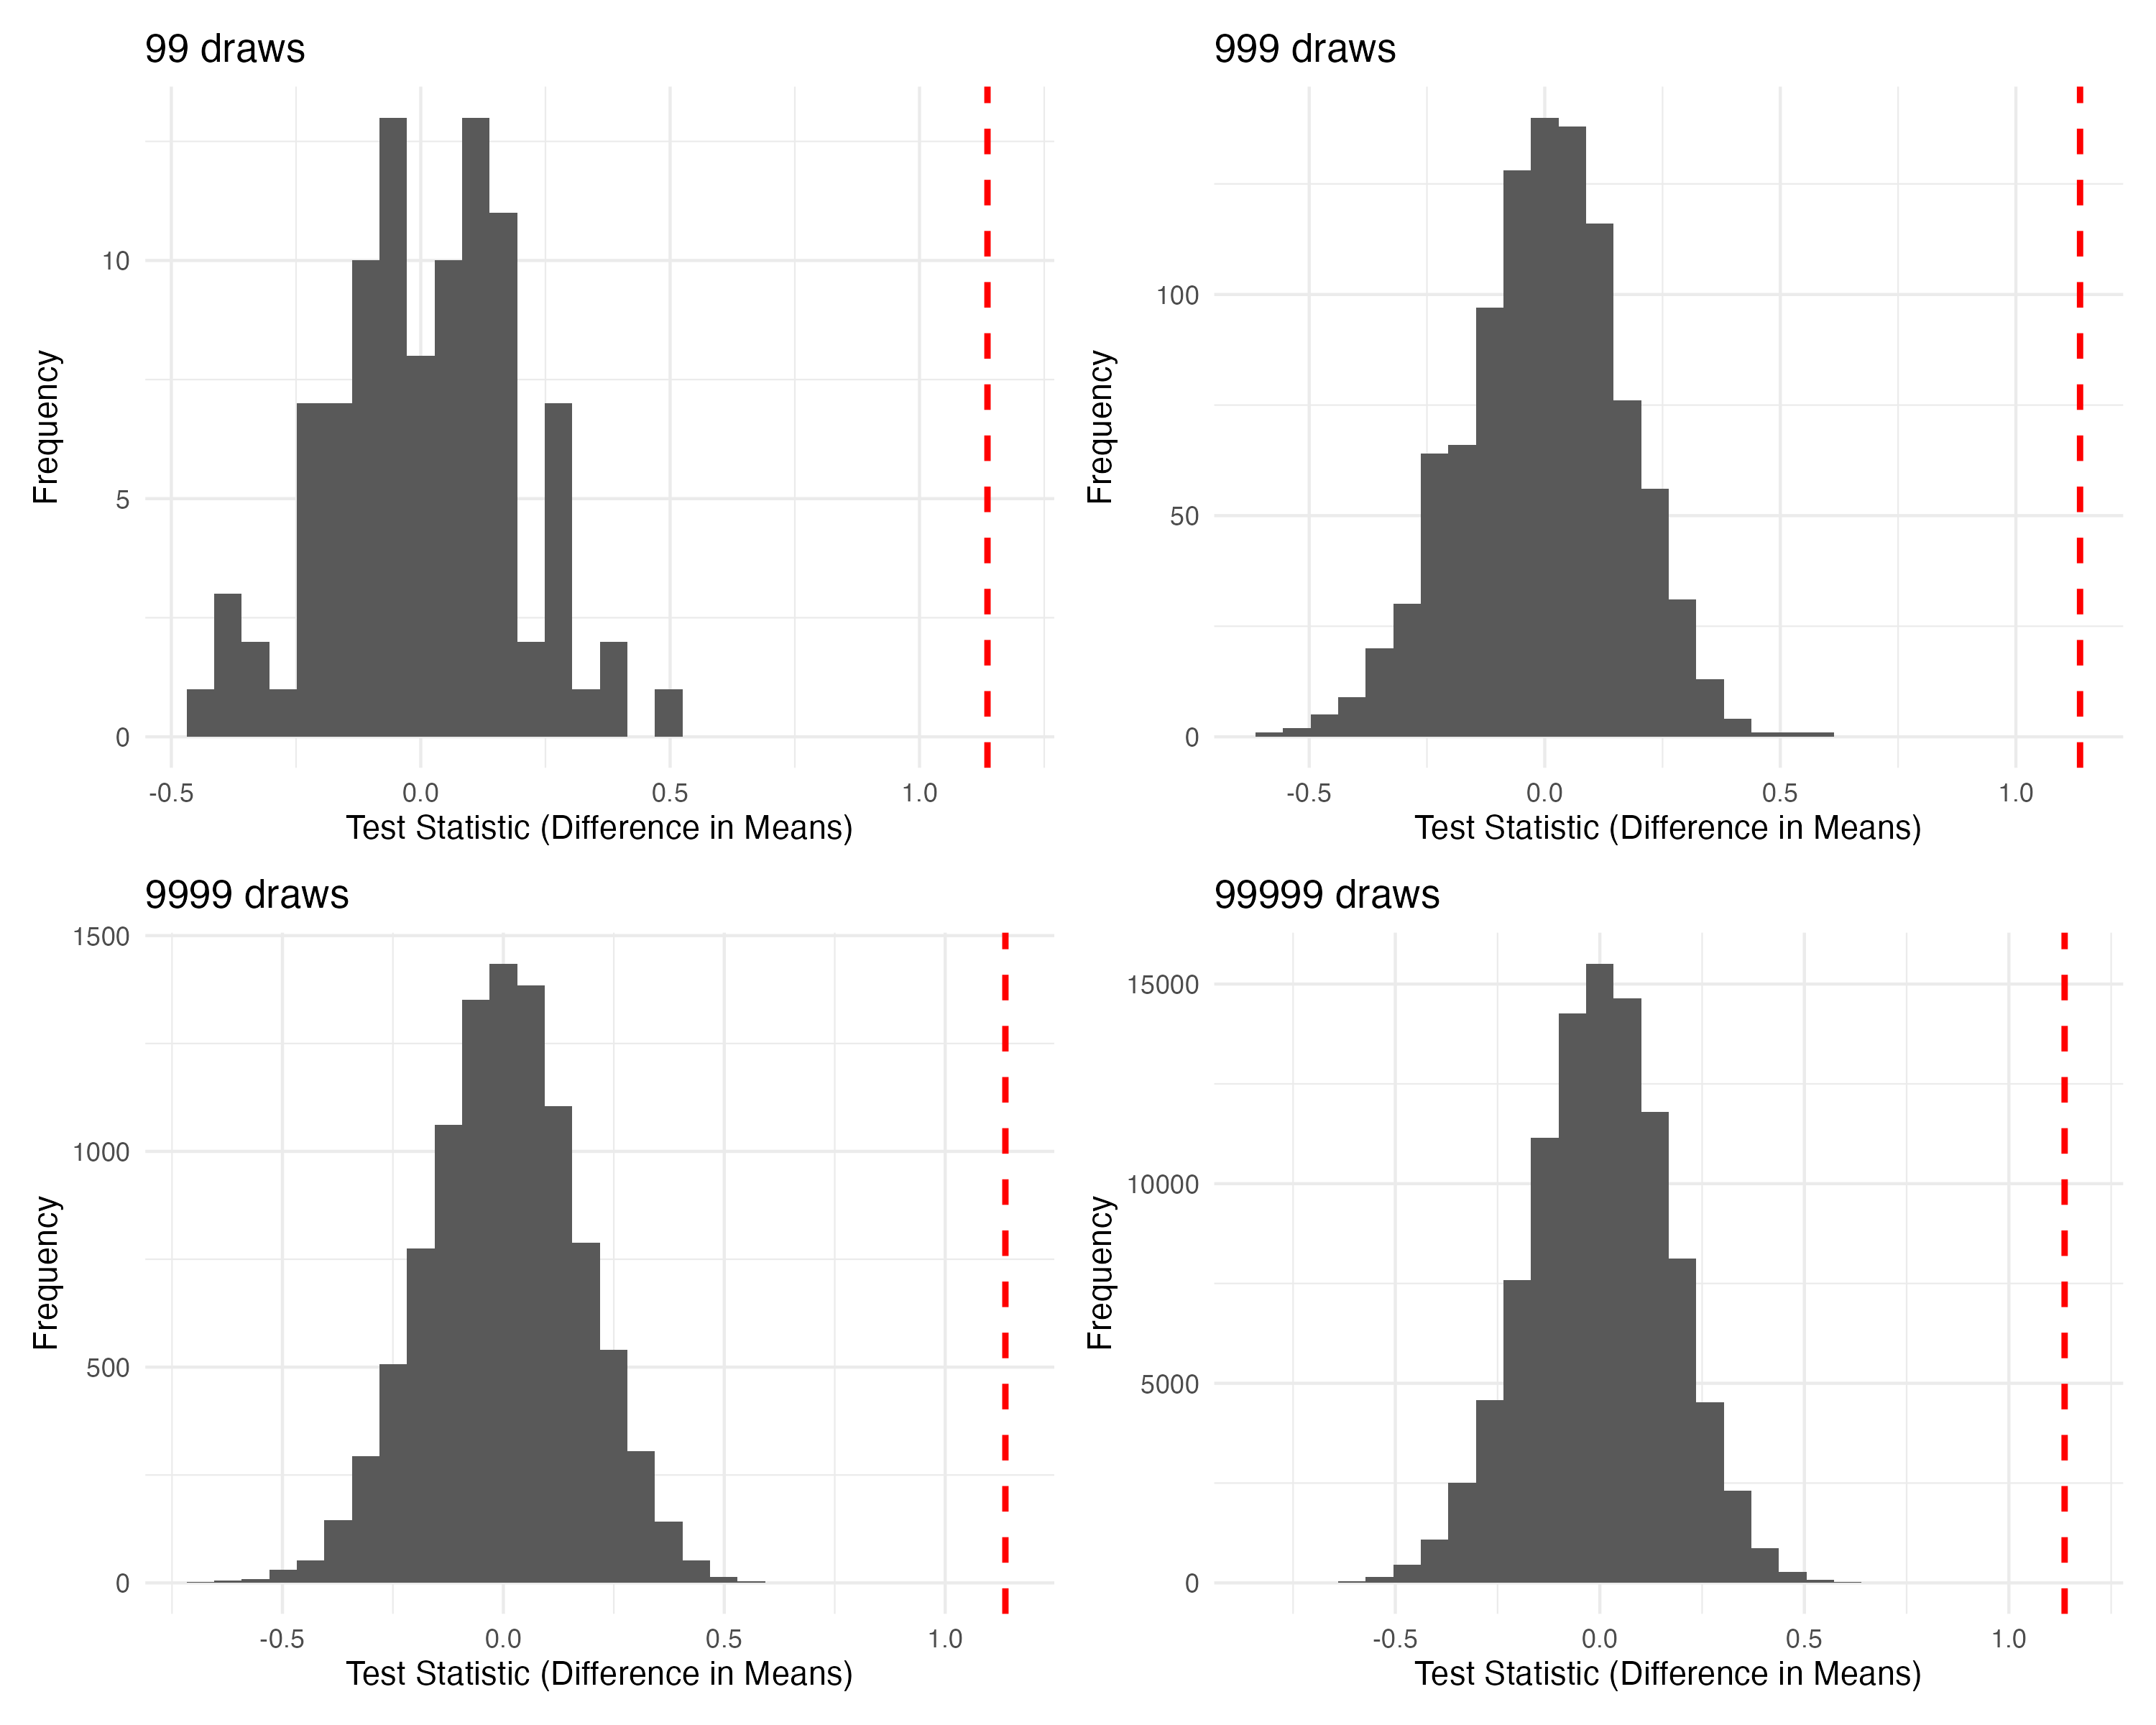
\includegraphics[width=\textwidth]{output/histograms_difference_in_means.png}
    \caption{\label{fig:dim}Difference-in-means by number of draws}
\end{figure}


Figure \ref{fig:dim} shows that the histograms of the test statistics under the null hypothesis of no treatment effect, generated from different numbers of random draws outside the actual draw we have. 
The red dashed line indicates the actual test statistic calculated from the observed data. 
Here, we can see that even 999 draws seem to be enough to get a reasonable approximation of the null distribution, and the p-value does not change much as we increase the number of draws. 
I remain trying different number of draws for problem I-(b) and (c) as well; however, if I had to choose a number, 999 seems to be sufficient.
The actual test statistic is 1.1362, and the p-value under 999 draws is 0.0000.\footnote{The p-values for each test statistic and number of draws are in table \ref{tab:p_values_all_draws}.}


\subsection*{(b) Difference-in-Medians}

\begin{figure}[h]
    \centering
    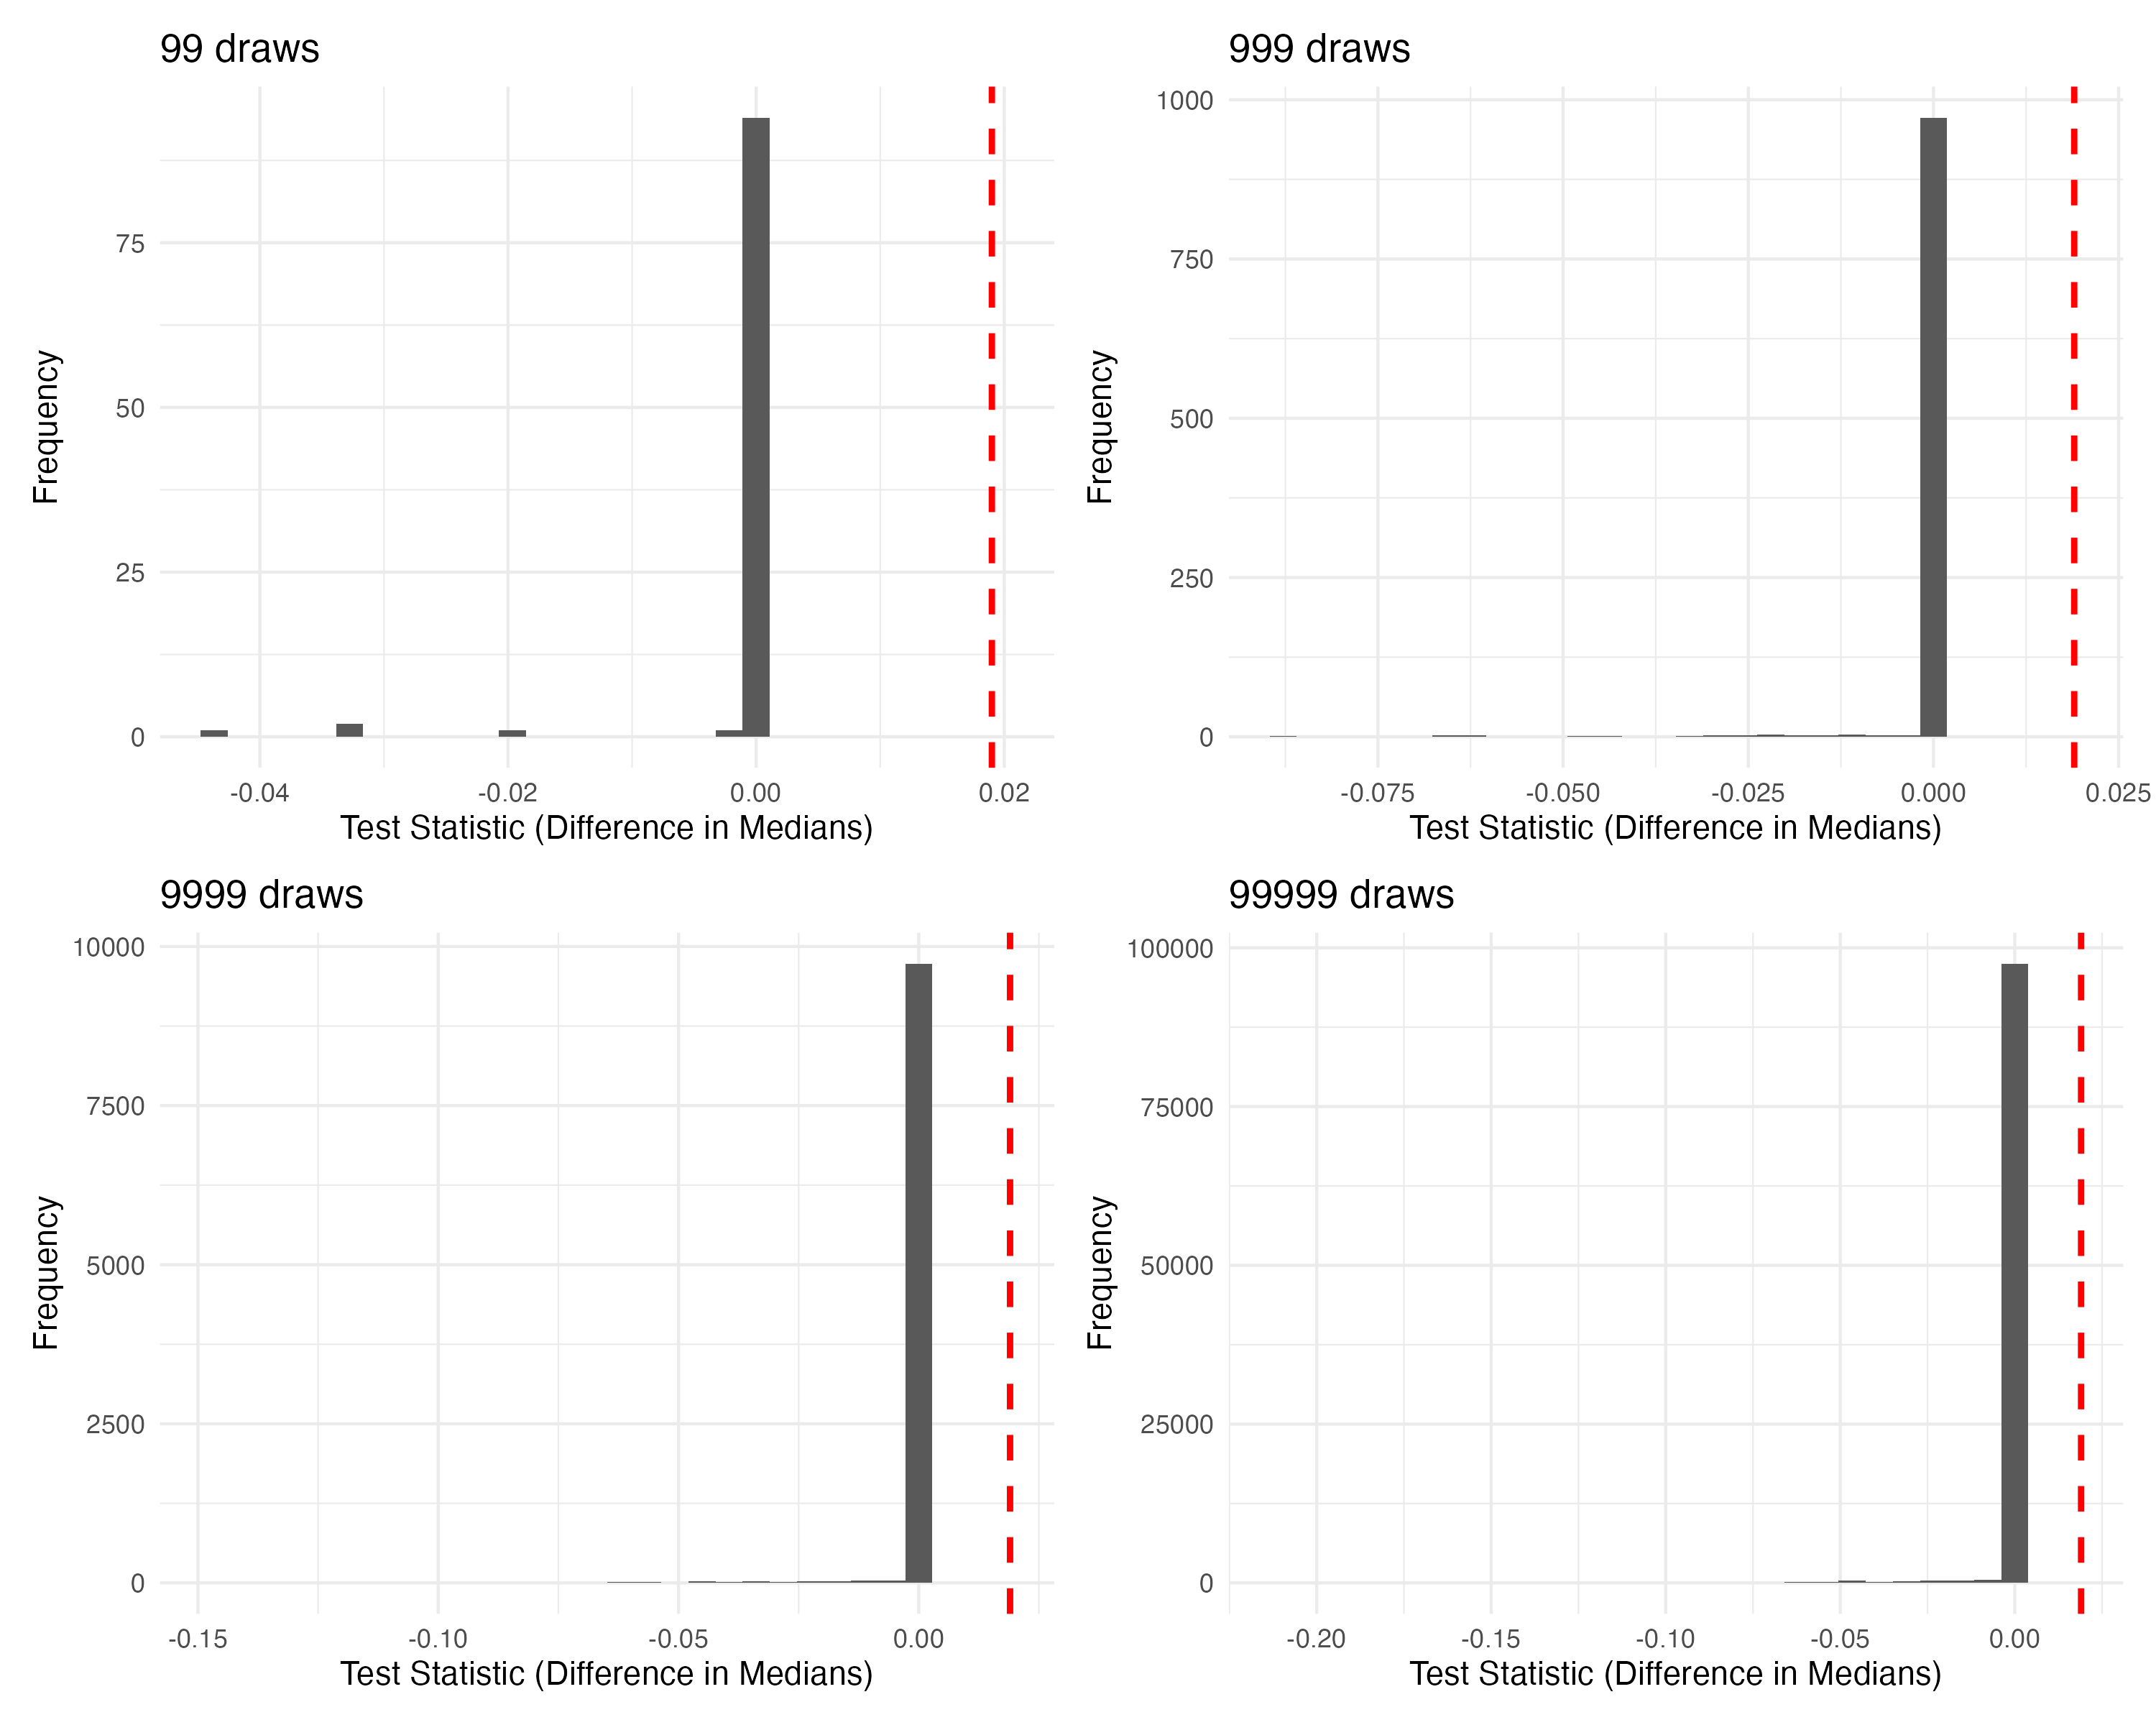
\includegraphics[width=\textwidth]{output/histograms_difference_in_medians.png}
    \caption{\label{fig:dim}Difference-in-medians by number of draws}
\end{figure}

With the difference-in-medians, we obtain the actual test statistic 0.019 and the p-value 0.017 under 999 draws(table \ref{tab:p_values_all_draws}).
This might not be the ideal test statistic to use, given that we have many zeros in the data(\verb|earnings1yr| has 52\% zeros).
\textcite{chen2024logs} explains how we can separate the treatment effects at the extensive margin and the intensive margin when the outcome is a weakly positive random variable, and \textcite{feng_comparison_2021} compares zero-inflated count models and hurdle models.
In this case, if the treatment does not strongly affect the extensive margin, the median of the two groups will not capture the treatment effect under a zero-inflated distribution.
To account for the zero-inflated nature of the data and the distinction between the extensive and intensive margins, we can use a hurdle model, which is demonstrated in the next section.


\subsection*{(c) Hurdle Estimates}

As for another statistic that we can use, we can use a hurdle model to account for the zero-inflated nature of the data.
The model I consider is as follows:

\begin{align}
P(Y_i > 0| W_i) &= \frac{1}{1+exp(-(\beta_0 + \beta_1 W_i + \beta_2 X_i + \beta_3 W_i \tilde{X}_i))} \label{eq:hurdle_prob}\\
\mathbb{E}\left[\log(Y_i)| W_i\right] &= \gamma_0 + \gamma_1 W_i + \gamma_2 X_i + \gamma_3 W_i \tilde{X}_i \label{eq:hurdle_mean}
\end{align}

where $\tilde{X}_i$ is the vector of demeaned covariates(high school diploma, female, age, single) excluding the treatment variable $W_i$.
Here, I allow the heterogeneity in the treatment effect by the observed covariates, and the covariates for the interaction term are demeaned so that $\beta_1$ and $\gamma_1$ capture the treatment effect for the individual with average characteristics.

The test statistic I consider from equations \ref{eq:hurdle_prob} and \ref{eq:hurdle_mean} is as follows:

\begin{align}
\hat{T} = \beta_1 + \gamma_1 \label{eq:hurdle}
\end{align}


\begin{figure}[ht]
    \centering
    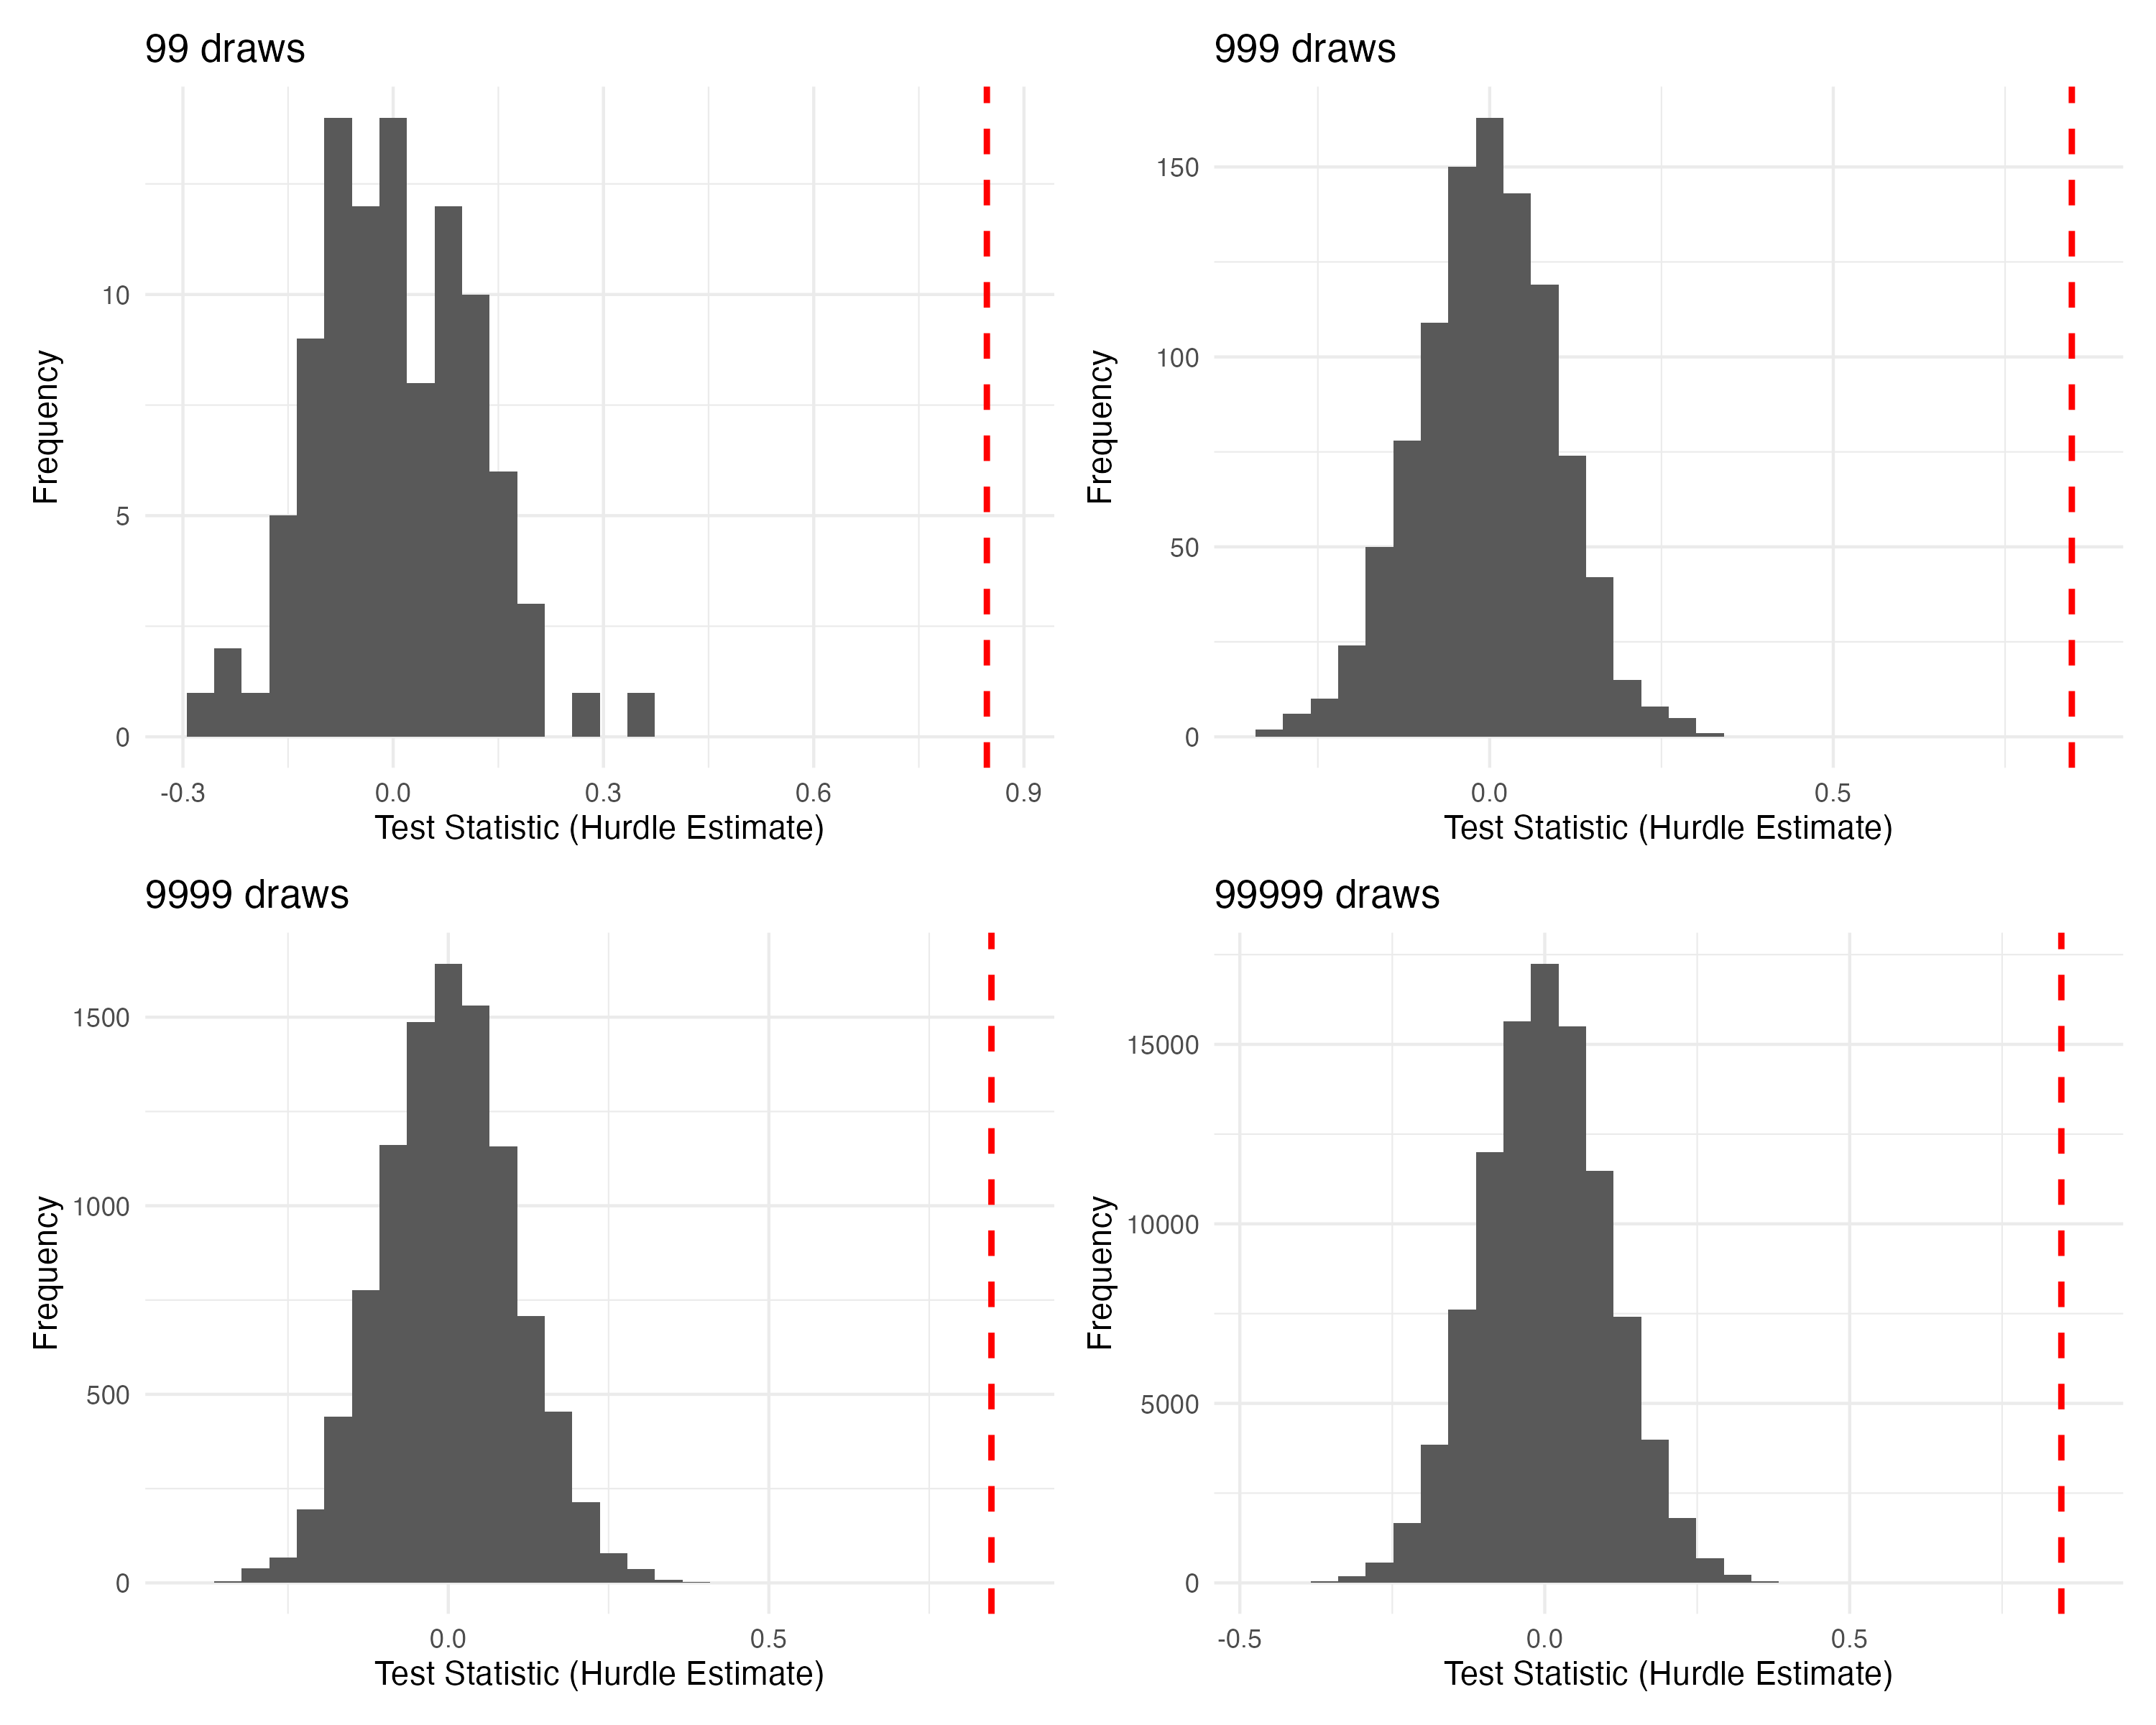
\includegraphics[width=\textwidth, height=8cm]{output/histograms_hurdle_model_estimate.png}
    \caption{\label{fig:hurdle}Hurdle model estimate by number of draws}
\end{figure}

Figure \ref{fig:hurdle} shows that the histograms of \ref{eq:hurdle} under the null hypothesis of no treatment effect, generated from different numbers of random draws outside the actual draw we have. 
The red dashed line indicates the actual test statistic calculated from the observed data. 
The actual test statistic is 0.8470, and the p-value under 999 draws is 0.0000(table \ref{tab:p_values_all_draws}).\footnote{One thing to note is that the distribution of the outliers in the median statistic is opposite to the previous median statistic under permutation. This is because although we have roughly 80\% of actual treated units, we assumed in this problem that 20\% are treated. However, the p-values are unaffected because it is the imbalance in the treatment and control groups that determines them, not the actual treated-to-control ratio.}

\subsection*{(d) Bernoulli Process}


Figure \ref{fig:bernoulli} shows the histograms of the three test statistics(mean, median, and hurdle) under the null hypothesis of no treatment effect from 999 draws, assuming a coin toss experiment with $p=0.2$.
The red dashed line indicates the actual test statistic calculated from the observed data. 

\begin{figure}[h]
    \centering
    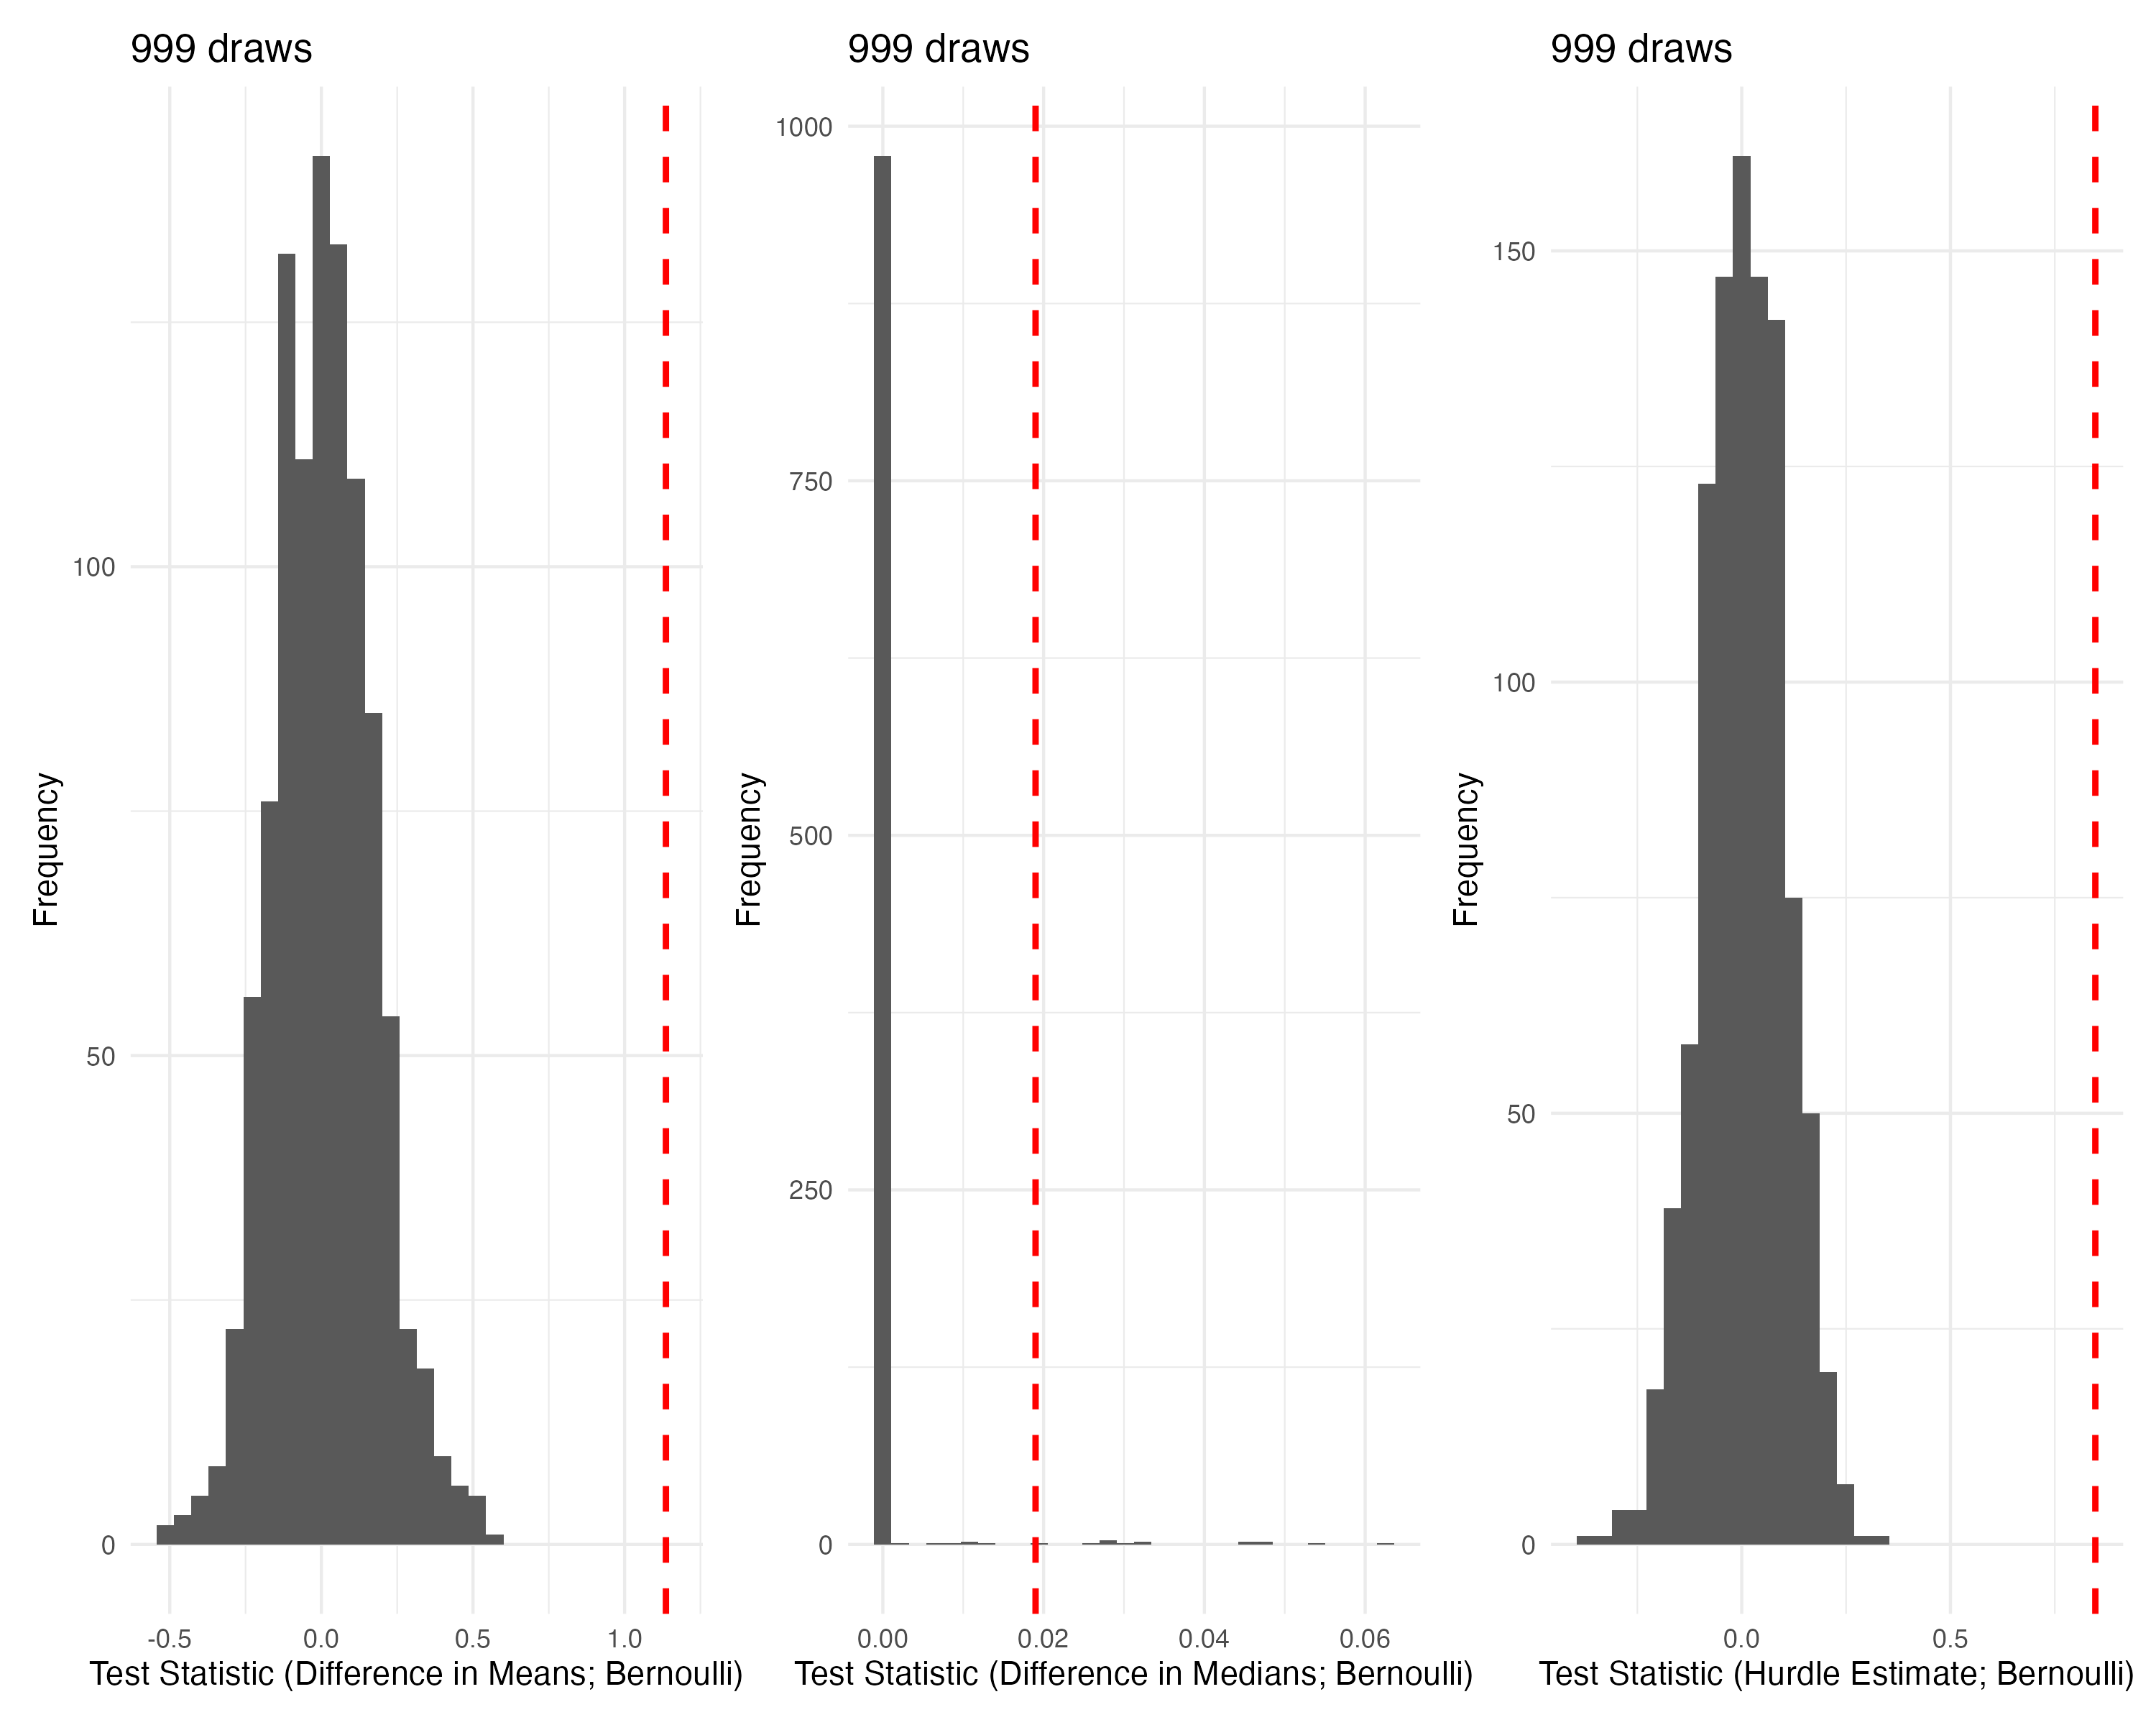
\includegraphics[width=\textwidth, height=5cm]{output/histograms_bernoulli.png}
    \caption{\label{fig:bernoulli}Bernoulli process}
\end{figure}


The p-values under 999 draws for all three test statistics are in table \ref{tab:p_values_bernoulli}, compared to the permutation p-values in the previous sections.
In this case, we have smaller p-values for the median statistic in the coin toss case. However, we cannot compare 
the other p-values directly since they are all zero. I believe the p-values of these two approaches can be very different if we have a large imbalance in the treatment and control groups or if the number of observations is small.
The reasons are discussed in Part \ref{sec:part_ii}.

\begin{table}[h]
    \centering
    \begin{tabular}{lcc}
        \toprule
        Test Statistic & Bernoulli & Permutation \\
        \midrule
        Mean & 0.0000 & 0.0000 \\
        Median & 0.0140 & 0.0170 \\
        Hurdle & 0.0000 & 0.0000 \\
        \bottomrule
    \end{tabular}
    \caption{\label{tab:p_values_bernoulli}P-values of the test statistics under different approaches(999 draws)}
\end{table}


\section{Part II}
\label{sec:part_ii}
\subsection*{(a) Theoretical Calculations}

In the current situation, with 49 treatment units and 51 control units, it is better to consider the permutation of the treatment status rather than considering the Bernoulli process that the experiment design actually followed.
This is not a universal rule, but in this case, since we have a balanced treatment and control groups, it is more appropriate to consider the permutation of the treatment status.
Assuming we use the usual test statistics such as difference-in-means or difference-in-medians, their variances usually increase with the imbalance of the treatment assignment.
If we were to consider the Bernoulli process, we also consider the test statistics under imbalanced treatment and control groups, and the specific values of these statistics will be more affected by the noise.
In other words, we will have more test statistics since we are considering $2^{100}$ possible treatment assignments instead of $\binom{100}{49}$ possible treatment assignments, but the extra test statistics will not have the same noise-to-signal ratio as the statistics under balanced treatment assignment.
However, if we limit to the case where we have 49 and 51 treated and control units, the variance of the test statistics are less likely to be affected by the noise.
Therefore, we should consider the permutation of the treatment status in this case.

\begin{table}[h]
    \centering
    \begin{tabular}[t]{rrr}
        \toprule
        simulations & permutation & bernoulli\\
        \midrule
        100 & 0.0099 & 0.0099\\
        1,000 & 0.0010 & 0.0020\\
        10,000 & 0.0010 & 0.0003\\
        50,000 & 0.0009 & 0.0009\\
        \bottomrule
    \end{tabular}
    \caption{\label{tab:tab:2asimulations}p-values: Permutation vs. Bernoulli}
    \label{tab:2asimulations}
\end{table}



Table \ref{tab:2asimulations} presents the p-values of the test statistics under the null hypothesis of no treatment effect based on the two different approaches: permutation and Bernoulli.
The DGP of this simulated data is as follows:

\begin{verbatim}
    Y0 <- rnorm(100, mean=50, sd=10)
    Y1 <- 1.1*Y0 + rnorm(100, mean=0, sd=1)
\end{verbatim}

where $Y_i(1)$ and $Y_i(0)$ are the potential outcomes for the $i$-th unit under the treatment and control scenarios, respectively.

We see that the p-values of the test statistics under the null hypothesis of no treatment effect are very close to each other, regardless of the number of random draws.


However, consider the situation where we ended up with 30 treated units and 70 control units.


In this case, our test statistic will be more likely to be affected by the noise.
Therefore, we should consider the Bernoulli process in this case.
Table \ref{tab:2asimulations(imbalanced)} is from the same DGP of the potential outcomes and Bernoulli process with $p=0.5$, but with 30 treated units and 70 control units.
That is, 

\begin{verbatim}
    Y0 <- rnorm(100, mean=50, sd=10)
    Y1 <- 1.1*Y0 + rnorm(100, mean=0, sd=1)
    W <- c(repeat(1, 30), repeat(0, 70))
    W <- shuffle(W)
    
    for (i in 1:num_simulations) {
        Wmock <- rbinom(100, 1, 0.5)  # random assignment with p=0.5
        diff_in_means <- mean(data$Y_obs[Wmock == 1]) -mean(data$Y_obs[Wmock == 0])
        test_statistics <- c(test_statistics, diff_in_means)
        }
    \end{verbatim}
    
    
\begin{table}[h]

\centering
\begin{tabular}[t]{rrr}
\toprule
simulations & permutation & bernoulli\\
\midrule
100 & 0.0198 & 0.0396\\
1,000 & 0.0539 & 0.0200\\
10,000 & 0.0439 & 0.0305\\
50,000 & 0.0447 & 0.0286\\
\bottomrule
\end{tabular}
\caption{\label{tab:tab:2asimulations(imbalanced)}p-values: Permutation vs. Bernoulli(30 T vs 70 C)}
\label{tab:2asimulations(imbalanced)}
\end{table}


In table \ref{tab:2asimulations(imbalanced)}, we see that the p-values of the test statistics under the null hypothesis of no treatment effect are significantly lower when we consider the Bernoulli process.
Therefore, it is better to consider the Bernoulli process when the resulted imbalance in treatment and control groups is large.


\appendix
\setcounter{figure}{0}                      
\setcounter{table}{0}                      
\renewcommand\thefigure{A.\arabic{figure}} 
\renewcommand\thetable{A.\arabic{table}} 

\begin{sidewaystable}[h]
    \centering
    \tiny
    
\begin{tabular}{lrrrrrrrrrrrrrrrr}
\toprule
variable & numNA & numZeros & fracZeros & mean & sd & min & max & 10\% & 20\% & 30\% & 40\% & 50\% & 90\% & 95\% & 99\% & 99.9\%\\
\midrule
educ & 0 & 598 & 0.0018 & 12.7699 & 3.2812 & 0.0000 & 20.0000 & 9.0000 & 11.0000 & 12.0000 & 12.0000 & 12.0000 & 17.0000 & 19.0000 & 20.000 & 20.0000\\
lwage & 0 & 3 & 0.0000 & 5.8999 & 0.6788 & -2.3418 & 10.5321 & 5.2343 & 5.5218 & 5.7243 & 5.8472 & 5.9525 & 6.5567 & 6.8004 & 7.274 & 7.9495\\
yob & 0 & 0 & 0.0000 & 34.6028 & 2.9050 & 30.0000 & 39.0000 & 30.0000 & 32.0000 & 33.0000 & 34.0000 & 35.0000 & 39.0000 & 39.0000 & 39.000 & 39.0000\\
\bottomrule
\end{tabular}

    \caption{\label{tab:summary_stats}Summary Statistics}
\end{sidewaystable}


\begin{sidewaystable}[h]
    \centering
    \tiny
    
\begin{tabular}{lrrrrrrrrrrrrrrrr}
\toprule
variable & numNA & numZeros & fracZeros & mean & sd & min & max & 10\% & 20\% & 30\% & 40\% & 50\% & 90\% & 95\% & 99\% & 99.9\%\\
\midrule
W & 0 & 1,036 & 1.0000 & 0.0000 & 0.0000 & 0.0000 & 0.0000 & 0.0000 & 0.0000 & 0.0000 & 0.0000 & 0.0000 & 0.0000 & 0.0000 & 0.0000 & 0.0000\\
earnings1yr & 0 & 679 & 0.6554 & 1.4493 & 3.4950 & 0.0000 & 34.5994 & 0.0000 & 0.0000 & 0.0000 & 0.0000 & 0.0000 & 5.1112 & 8.6316 & 16.3443 & 28.6786\\
earnings4yr & 0 & 678 & 0.6544 & 3.0354 & 6.8941 & 0.0000 & 51.5277 & 0.0000 & 0.0000 & 0.0000 & 0.0000 & 0.0000 & 11.7650 & 17.7781 & 31.8940 & 51.4125\\
hs\_diploma & 0 & 494 & 0.4768 & 0.5232 & 0.4997 & 0.0000 & 1.0000 & 0.0000 & 0.0000 & 0.0000 & 0.0000 & 1.0000 & 1.0000 & 1.0000 & 1.0000 & 1.0000\\
female & 0 & 130 & 0.1255 & 0.8745 & 0.3314 & 0.0000 & 1.0000 & 0.0000 & 1.0000 & 1.0000 & 1.0000 & 1.0000 & 1.0000 & 1.0000 & 1.0000 & 1.0000\\
\addlinespace
age & 0 & 0 & 0.0000 & 33.8205 & 8.3839 & 15.0000 & 66.0000 & 25.0000 & 28.0000 & 29.0000 & 31.0000 & 33.0000 & 45.0000 & 49.0000 & 58.0000 & 62.9650\\
child & 0 & 865 & 0.8349 & 0.1651 & 0.3714 & 0.0000 & 1.0000 & 0.0000 & 0.0000 & 0.0000 & 0.0000 & 0.0000 & 1.0000 & 1.0000 & 1.0000 & 1.0000\\
single & 0 & 126 & 0.1216 & 0.8784 & 0.3270 & 0.0000 & 1.0000 & 0.0000 & 1.0000 & 1.0000 & 1.0000 & 1.0000 & 1.0000 & 1.0000 & 1.0000 & 1.0000\\
hs\_diploma\_dm & 0 & 0 & 0.0000 & 0.0000 & 0.4997 & -0.5232 & 0.4768 & -0.5232 & -0.5232 & -0.5232 & -0.5232 & 0.4768 & 0.4768 & 0.4768 & 0.4768 & 0.4768\\
female\_dm & 0 & 0 & 0.0000 & -0.0050 & 0.3314 & -0.8795 & 0.1205 & -0.8795 & 0.1205 & 0.1205 & 0.1205 & 0.1205 & 0.1205 & 0.1205 & 0.1205 & 0.1205\\
\addlinespace
age\_dm & 0 & 0 & 0.0000 & 0.1803 & 8.3839 & -18.6402 & 32.3598 & -8.6402 & -5.6402 & -4.6402 & -2.6402 & -0.6402 & 11.3598 & 15.3598 & 24.3598 & 29.3248\\
single\_dm & 0 & 0 & 0.0000 & 0.0125 & 0.3270 & -0.8658 & 0.1342 & -0.8658 & 0.1342 & 0.1342 & 0.1342 & 0.1342 & 0.1342 & 0.1342 & 0.1342 & 0.1342\\
\bottomrule
\end{tabular}

    \caption{\label{tab:summary_stats(control_group)}Summary Statistics}
\end{sidewaystable}


\begin{sidewaystable}[h]
    \centering
    \tiny
    
\begin{tabular}{lrrrrrrrrrrrrrrrr}
\toprule
variable & numNA & numZeros & fracZeros & mean & sd & min & max & 10\% & 20\% & 30\% & 40\% & 50\% & 90\% & 95\% & 99\% & 99.9\%\\
\midrule
W & 0 & 0 & 0.0000 & 1.0000 & 0.0000 & 1.0000 & 1.0000 & 1.0000 & 1.0000 & 1.0000 & 1.0000 & 1.0000 & 1.0000 & 1.0000 & 1.0000 & 1.0000\\
earnings1yr & 0 & 2,179 & 0.4971 & 2.5855 & 5.2141 & 0.0000 & 60.0000 & 0.0000 & 0.0000 & 0.0000 & 0.0000 & 0.0190 & 8.4014 & 11.7693 & 23.5991 & 56.8758\\
earnings4yr & 0 & 2,574 & 0.5873 & 4.2677 & 8.3822 & 0.0000 & 60.0000 & 0.0000 & 0.0000 & 0.0000 & 0.0000 & 0.0000 & 15.3113 & 22.4685 & 38.1191 & 60.0000\\
hs\_diploma & 0 & 2,090 & 0.4768 & 0.5232 & 0.4995 & 0.0000 & 1.0000 & 0.0000 & 0.0000 & 0.0000 & 0.0000 & 1.0000 & 1.0000 & 1.0000 & 1.0000 & 1.0000\\
female & 0 & 523 & 0.1193 & 0.8807 & 0.3242 & 0.0000 & 1.0000 & 0.0000 & 1.0000 & 1.0000 & 1.0000 & 1.0000 & 1.0000 & 1.0000 & 1.0000 & 1.0000\\
\addlinespace
age & 0 & 0 & 0.0000 & 33.5975 & 8.1511 & 16.0000 & 70.0000 & 24.0000 & 27.0000 & 29.0000 & 31.0000 & 33.0000 & 44.0000 & 49.0000 & 57.0000 & 61.6180\\
child & 0 & 3,667 & 0.8366 & 0.1634 & 0.3697 & 0.0000 & 1.0000 & 0.0000 & 0.0000 & 0.0000 & 0.0000 & 0.0000 & 1.0000 & 1.0000 & 1.0000 & 1.0000\\
single & 0 & 601 & 0.1371 & 0.8629 & 0.3440 & 0.0000 & 1.0000 & 0.0000 & 1.0000 & 1.0000 & 1.0000 & 1.0000 & 1.0000 & 1.0000 & 1.0000 & 1.0000\\
hs\_diploma\_dm & 0 & 0 & 0.0000 & 0.0000 & 0.4995 & -0.5232 & 0.4768 & -0.5232 & -0.5232 & -0.5232 & -0.5232 & 0.4768 & 0.4768 & 0.4768 & 0.4768 & 0.4768\\
female\_dm & 0 & 0 & 0.0000 & 0.0012 & 0.3242 & -0.8795 & 0.1205 & -0.8795 & 0.1205 & 0.1205 & 0.1205 & 0.1205 & 0.1205 & 0.1205 & 0.1205 & 0.1205\\
\addlinespace
age\_dm & 0 & 0 & 0.0000 & -0.0426 & 8.1511 & -17.6402 & 36.3598 & -9.6402 & -6.6402 & -4.6402 & -2.6402 & -0.6402 & 10.3598 & 15.3598 & 23.3598 & 27.9778\\
single\_dm & 0 & 0 & 0.0000 & -0.0030 & 0.3440 & -0.8658 & 0.1342 & -0.8658 & 0.1342 & 0.1342 & 0.1342 & 0.1342 & 0.1342 & 0.1342 & 0.1342 & 0.1342\\
\bottomrule
\end{tabular}

    \caption{\label{tab:summary_stats(treated_group)}Summary Statistics}
\end{sidewaystable}


\begin{table}[h]
\centering\begingroup

\begin{tabular}{lcccc}
\toprule
Test Statistic & 99 Draws & 999 Draws & 9999 Draws & 99999 Draws\\
\midrule
Difference in Means & 0.0000 & 0.000 & 0.0000 & 0.0000\\
Difference in Medians & 0.0404 & 0.017 & 0.0166 & 0.0162\\
Hurdle Estimate & 0.0000 & 0.000 & 0.0000 & 0.0000\\
\bottomrule
\end{tabular}
\endgroup{}

\caption{\label{tab:p_values_all_draws}P-values of the test statistics under the null hypothesis of no treatment effect by number of draws}
\end{table}



\printbibliography

\end{document}